% article example for classicthesis.sty
\documentclass[10pt,a4paper]{article} % KOMA-Script article scrartcl
\usepackage{import}
\usepackage{xifthen}
\usepackage{pdfpages}
\usepackage{transparent}
\newcommand{\incfig}[1]{%
    \def\svgwidth{\columnwidth}
    \import{./figures/}{#1.pdf_tex}
}
\usepackage{lipsum}     %lorem ipsum text
\usepackage{titlesec}   %Section settings
\usepackage{titling}    %Title settings
\usepackage[margin=10em]{geometry}  %Adjusting margins
\usepackage{setspace}
\usepackage{listings}
\usepackage{amsmath}    %Display equations options
\usepackage{amssymb}    %More symbols
\usepackage{xcolor}     %Color settings
\usepackage{pagecolor}
\usepackage{mdframed}
\usepackage[spanish]{babel}
\usepackage[utf8]{inputenc}
\usepackage{longtable}
\usepackage{multicol}
\usepackage{graphicx}
\graphicspath{ {./Images/} }
\setlength{\columnsep}{1cm}

% ====| color de la pagina y del fondo |==== %
\pagecolor{black}
\color{white}



\begin{document}
    %========================{TITLE}====================%
    \title{{  Apuntes temas de geometría de la muestra  }}
    \author{{Rodrigo Castillo}}
    \date{\today}

    \maketitle


     % ====| Loguito |==== %
    
\includegraphics[width=0.1\linewidth]{negro_cara.png}
    %=======================NOTES GOES HERE===================%

    \section{geometría de la muestra}
        \begin{itemize}
            \item {se tiene una matriz de p variables y n observacones, entonces
                cada fila de la matriz representa una observacion multivariable}
            \item {el conjunto de medias a menudo es una realizacion particular de
                lo que podria haberse observado}
            \item {n mediciones cada una tiene p componentes}
        \end{itemize}

        los datos se pueden graficar de dos formas ...

        \begin{enumerate}
            \item {n puntos en el espacio p dimensional}
            \item {p puntos en el espacio n dimensional}
        \end{enumerate}

        \begin{itemize}
            \item {el diagrama de dispercion en de n puntos p-dimensional
                proporciona informacion sobre las ubicaciones y la variabilidad
            de los puntos}
            \item {si los puntos se consideran esferas solidas, el vector de la
                media muestal $ \hat{x}   $  es el \color{red} centro de
                equilibrio \color{white} }
            \item {la variabilidad ocurre en mas de una direccion , la matriz
                de varianza $ S_n  $ cuantifica eso}
            \item {cuando p es mayor que 3 no se puede hacer nada}
            \item {la consideracion de los datos como $ n  $  puntos en $ p  $
                dimensiones proporciona conocimientos que no se ven en las
                expresiones algebraicas}
            \item {los conceptos ilustraos en $ p=2  $  o $ p=3  $  siguen
                siendo validos}

        \end{itemize}
        \begin{figure}[h!]
            \centering
            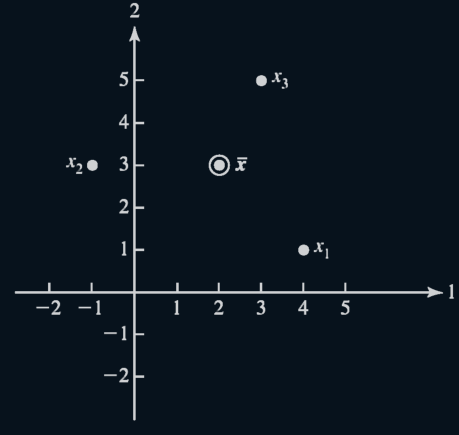
\includegraphics[width=0.4\linewidth]{grafica.png}
            \caption{Grafica tomando $ n=3  $  en $ p=2  $ dimensiones }
            \label{fig:grafica}
        \end{figure}

        \begin{figure}[h!]
            \centering
            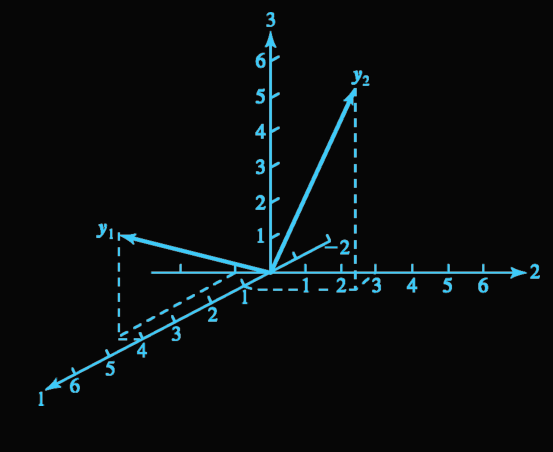
\includegraphics[width=0.4\linewidth]{grafica2.png}
            \caption{$ p=2  $ vectores en un espacion $ n=3  $  dimensiones}
            \label{fig:grafica2}
        \end{figure}
        \newpage





    \section{Muestras Aleatorias}
        es lo mismo pero ahora los valores son aleatorios y blah blah blah


















    %=======================NOTES ENDS HERE===================%

    % bib stuff
    \nocite{*}
    \addtocontents{toc}{{}}
    \addcontentsline{toc}{section}{\refname}
    \bibliographystyle{plain}
    \bibliography{../Bibliography}
\end{document}
